%%%--------------------------------------------------------------------------------------------
\documentclass[a4paper, jou, natbib]{apa6}
\usepackage[english]{babel}
\usepackage[utf8x]{inputenc}
\usepackage{mathtools}
\usepackage{amssymb}
\usepackage{graphicx}
\usepackage[colorinlistoftodos]{todonotes} 
\usepackage{etoolbox}

% \newtoggle{jou}
% \toggletrue{jou}
% \togglefalse{jou}

% \usepackage{lineno}

\title{The Effect of Episodic Retrieval on Inhibition in Task Switching}
\shorttitle{Episodic Retrieval \& Inhibition}
\author{James A. Grange, Agnieszka Kowalczyk, and Rory O'Loughlin}
\affiliation{School of Psychology, Keele University, UK}

\note{{\bf Word Count:} x,xxx (Main body, not including abstract or references.)}
% \note{{\bf Under Review---Please, no direct quotes.}}

% command to insert editing comments or track changes
\newcommand{\jg}[1]{\textcolor{blue}{$^{\textrm{}}${#1}}}

%command for R symbol
\newcommand{\R}{R}

\authornote{Please address correspondence to James A. Grange, School of Psychology, Dorothy Hodgkin Building, Keele University, Keele, UK, ST5 5BG. Email: grange.jim@gmail.com. All raw data and analysis code are available to download at http://bit.ly/1l22EUV.}

\leftheader{Grange}


\abstract{.}

\keywords{Task switching; inhibition, episodic retrieval, cognitive control}

\begin{document}
\maketitle

%----------------------
\section{Introduction}



\begin{figure}
\begin{center}
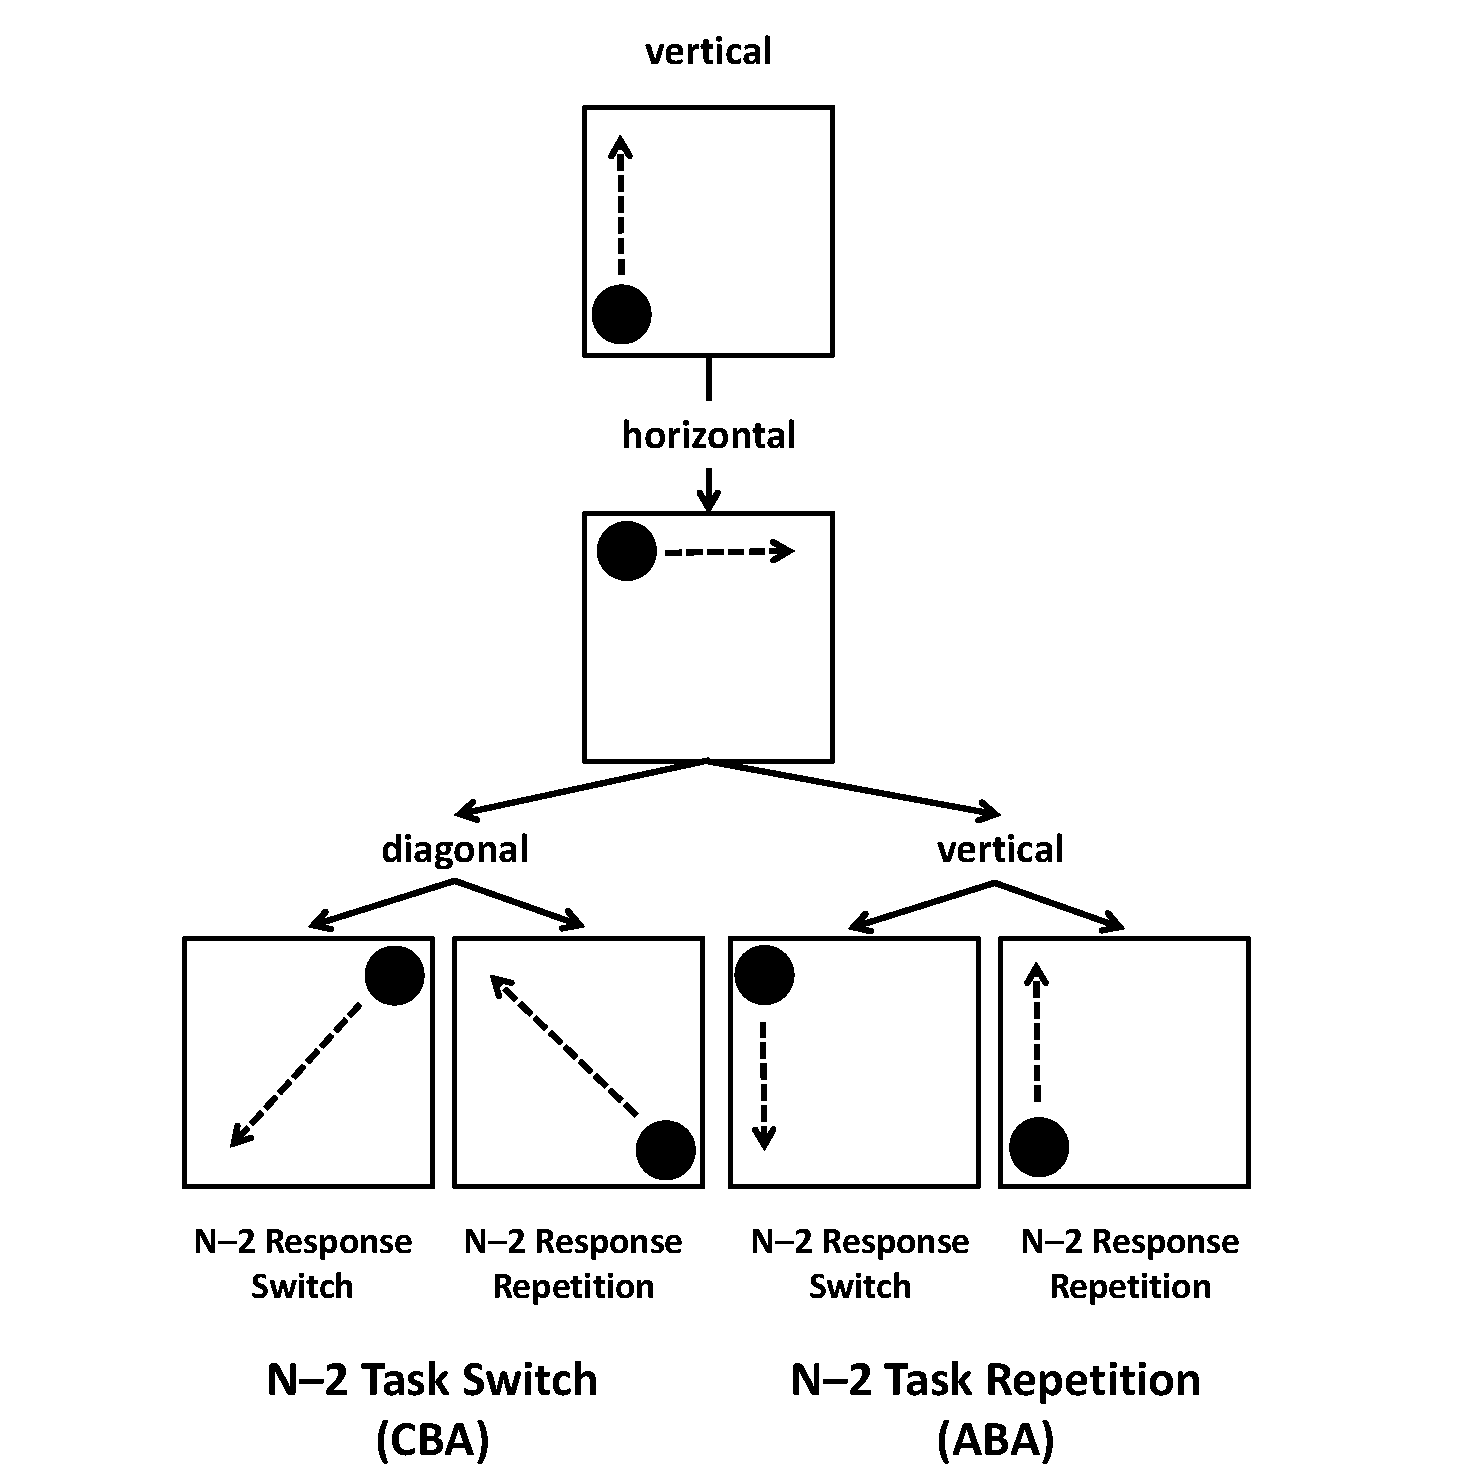
\includegraphics[width = 0.5 \textwidth]{Images/mayrExperiment.pdf}
\caption{Schematic overview of Mayr's (2002) experimental procedure. See text for details.}
\label{fig:mayrExperiment}
\end{center}
\end{figure}


\section{Changes from Mayr's (2002) Experiment}
List the main changes we made in this experiment compared to that of \cite{Mayr2002}.

%----------------------
\section{Method}

\subsection{Participants}
All participants were recruited via the participant panel run by the School of Psychology at Keele University. All participants were first year undergraduates participating in exchange for partial course credit. Our final sample comprised 76 participants. Three additional participants were removed before analysis due to failure to maintain accuracy levels above 90\%.

Our sample size was determined via optional stopping. We used Sequential Bayes Factors \citep{Schoenbrodtinpress} to determine our stopping rule for participant recruitment. We were interested in establishing the presence or absence of an interaction between task sequence (ABA vs. CBA) and response repetition (repetition vs. switch). For the purposes of our stopping rule, this can be expressed as a default within-subjects Bayesian t-test \citep{Rouder2009} comparing n--2 repetition costs for response repetitions and response switches. The Bayes Factor (denoted $BF_{10}$) quantifies the relative evidence provided by the data in favour of an alternative hypothesis (i.e., n--2 repetition costs are different) over a null hypothesis (i.e., n--2 repetition costs are equivalent). We conducted a Bayesian t-test on the data collected until the criteria for our a priori stopping rule were met. Specifically, our stopping rule required at least 20 participants; we continued data collection until $BF_{10}$ > 6 (constituting support for the alternative hypothesis) or $BF_{10}$ < 1/6 (constituting support for the null). \cite{Schoenbrodtinpress} demonstrated that a stopping rule of $BF_{10}$ > 6 (or $BF_{10}$ < 1/6) provided the best balance between type 1 and type 2 error, and was their recommended value for studies utilising Sequential Bayes Factors. 

\subsection{Apparatus \& Stimuli}
Stimuli were presented on an xin. monitor connected to a PC running E-Prime v. 2.0 software. The stimulus display consisted of an 8cm by 8cm square frame. A black circle (diameter = 1cm) served as the trial stimulus. Possible cues were the words ``horizontal'', ``vertical'', or ``diagonal'', and were presented in black font (enter font details here) directly above the stimulus frame. Responses were collected via a 1-ms precise USB keyboard.

\subsection{Procedure}
On each trial a cue was presented above the frame for xxms. After this time, the circle stimulus appeared in one of the four corners of the frame. The cue remained on the screen during stimulus presentation. The task required participants to mentally make a spatial transformation of the stimulus' location according to the rule dictated by the task cue, and to make a spatially-congruent response to this translated location. For example, if the stimulus was in the top-right corner, the participant would need to make a top-left response if the task was ``horizontal'', a bottom-right response if the task was ``vertical'', and a bottom-left response if the task was ``diagonal''. Responses were made on the numerical part of the keyboard, using the ``4'', ``5'', ``1'', and ``2'' keys for top-left, top-right, bottom-left, and bottom-right responses respectively. Participants were asked to respond as quickly and as accurately as possible. Once a response was registered, the frame was cleared for a response--cue interval of xxms, after which time a new cue appeared for the next trial. The cue for the next trial was chosen randomly with the constraint that task repetitions could not occur (cf., Mayr, 2002); the stimulus location was chosen randomly with no constraints on each trial. If participants made an error, the word ``Error!'' appeared in red for xxms above the stimulus frame (in the cue's position).

Participants were presented with xx trials as practice (which could be repeated upon request). The main experiment presented x blocks of x trials. 

\subsection{Design}
The experiment manipulated two factors in a fully-related design: \emph{Task Sequence} (n--2 task repetition [ABA] vs. n--2 task switch [CBA]) and \emph{Response Repetition} (n--2 response repetition vs. n-- response switch). The dependent variables were response time (RT) in milliseconds (ms) and percent accuracy (\%).


%----------------------
\section{Results}

\subsection{Data trimming}
Participants who failed to maintain session-wise accuracy above 90\% were immediately discarded from analysis. For response time analysis, the first two trials from each block were removed, as were error trials and the two trials following an error. Response times were trimmed by removing all RTs faster than 150ms, as well as any RTs slower than 2.5 standard deviations above the mean for each participant for each cell of the experimental design. 

\subsection{Standard Analysis}
Mean RTs and error rates can be seen in Table \ref{tab:behaviouralData}.


\begin{table*}[htbp]
\centering
\caption{Response times (RT) in milliseconds (ms) and accuracy (in percent) for ABA and CBA task sequences for response repetitions and response switches.}
\label{my-label}
\begin{tabular}{lccccc}
\hline
                    & \multicolumn{5}{c}{Task Sequence}                       \\ \cline{2-6} 
                    & \multicolumn{2}{c}{ABA}   &  & \multicolumn{2}{c}{CBA}  \\ \cline{2-3} \cline{5-6} 
                    & RT (ms)   & Accuracy (\%) &  & RT (ms)  & Accuracy (\%) \\ \hline
Response Repetition & 1000 (28) & 96.20 (0.39)  &  & 952 (28) & 96.36 (0.39) \\
Response Switch     & 1050 (29) & 95.02 (0.35)  &  & 964 (28) & 95.81 (0.34) \\ \hline
\end{tabular}
\label{tab:behaviouralData}
\end{table*}

Response times were analysed via a two factor repeated measures analysis of variance (ANOVA) with the factors as described in \emph{Design}. There was a significant main effect of \emph{Sequence}, with slower RTs to ABA sequences (1,025ms) than to CBA sequences (958ms), $F$(1, 75) = 94.14, $p$<.001, $\eta_g^2$ = .018.  There was also a significant main effect of \emph{Response Sequence}, with faster RTs to response repetitions (976ms) than to response switches (1,007ms), $F$(1, 75) = 18.21, $p$<.001, $\eta_g^2$ = .004.  Critically, there was a significant interaction of both factors, $F$(1, 75) = 9.60, $p$<.01, $\eta_g^2$ = .001. The n--2 repetition cost was 48ms for response repetitions [t(75) = 4.2, $p$<.001] and 86ms for response switches [t(75) = 13.0, $p$<.001].

\subsection{Sequential Bayes Factors}
The progression of the Sequential Bayes Factor is shown in Figure \ref{fig:bayesFactor}. We stopped data collection after 76 participants, as at this point the criteria for our stopping rule had been reached. 

\begin{figure}
\begin{center}
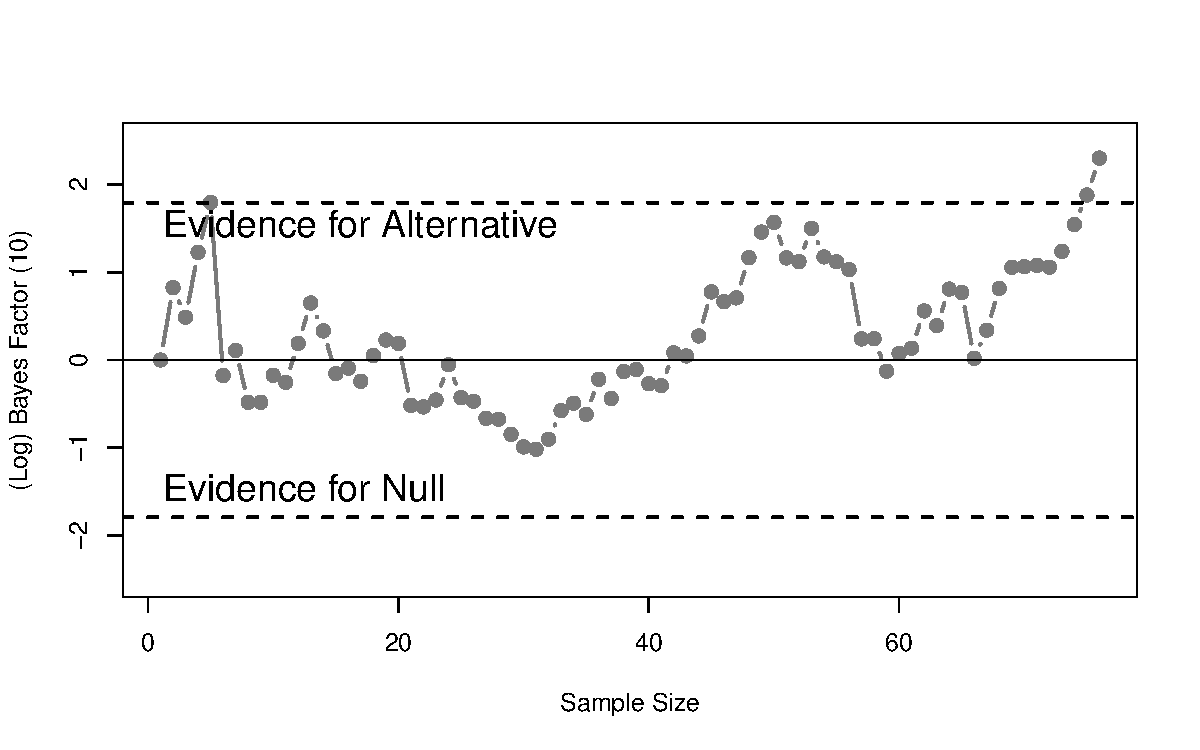
\includegraphics[width = 0.5\textwidth]{Images/bayesFactor.pdf}
\caption{Progression of the Sequential Bayes Factor [expressed as log($BF_{10}$)] as sample size increased. The criteria for a priori stopping rules are shown as dotted horizontal lines.}
\label{fig:bayesFactor}
\end{center}
\end{figure}

The final Bayes Factor for the difference of n--2 repetition costs for response repetitions and response switches was $BF_{10}$ = 9.974, which suggests that the alternative hypothesis is about 10 times more likely given than the data, which provides strong support that n--2 repetition costs are influenced by response repetitions.





%----------------------
\section{Discussion}

\subsection{Robustness of Recruitment Order on the Sequential Bayes Factor}
The progression of the Bayes Factor as sample size increased (Figure \ref{fig:bayesFactor}) appeared to provide slight evidence in favour of the null between sample sizes of 30 and 40, although the criterion for stopping was not reached. One might wonder, therefore, whether had a few more participants been recruited to the experiment showing a null interaction would we have stopped data collection and found evidence in favour of the null?

We wanted to assess how robust our stopping rule was to this apparent early evidence in favour of the null. Specifically, we were interested in whether our stopping rule in favour of the null would have been met had the participants been recruited in a different order. To assess this, we generated 50 random recruitment orders from our data set, and plotted the Sequential Bayes Factors for each recruitment order. If our findings are robust against recruitment order, the stopping rule in favour of the null should be rarely (if ever) met.  The results of this simulation are shown in Figure \ref{fig:recruitmentOrder}; each line represents the Sequential Bayes Factor for a random recruitment order. As can be seen, the stopping criterion in favour of the null is never met, suggesting our results are indeed robust to recruitment order.


\begin{figure}
\begin{center}
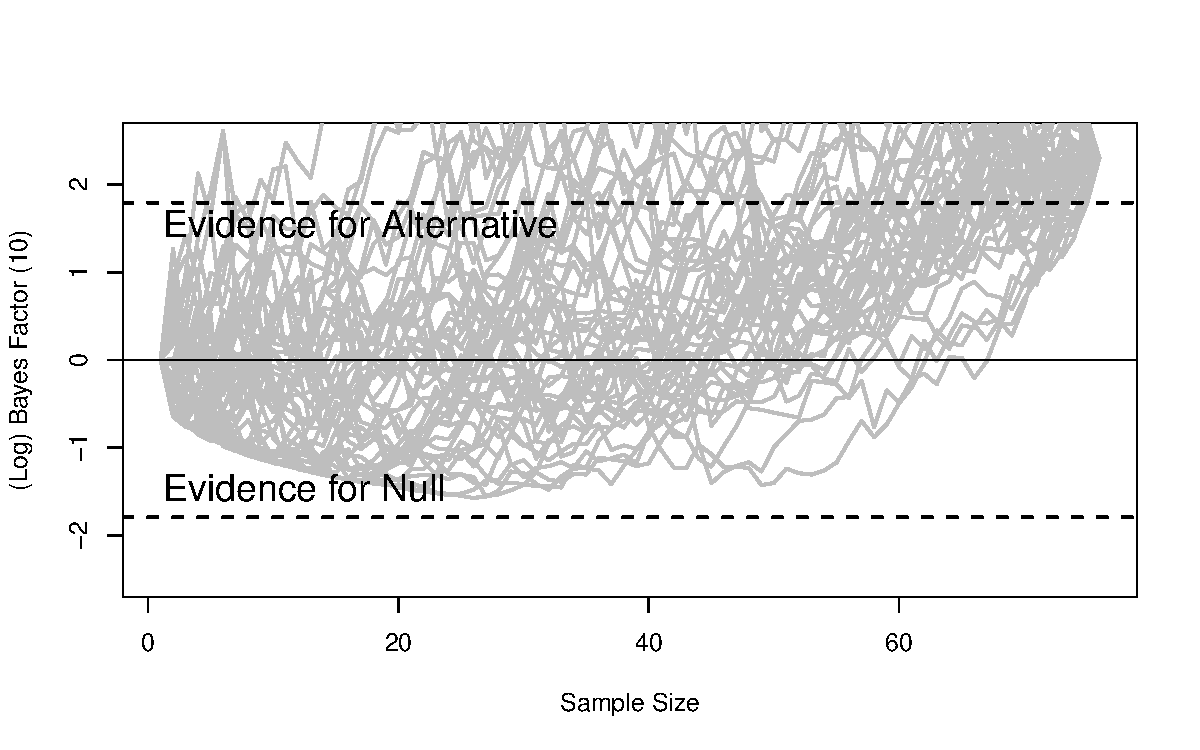
\includegraphics[width = 0.5 \textwidth]{Images/recruitmentOrder.pdf}
\caption{Simulated progression of the Sequential Bayes Factors for a random set of 50 different recruitment orders for the current data set. See text for details.}
\label{fig:recruitmentOrder}
\end{center}
\end{figure}








%%%--------------------------------------------------------------------------------------------


%%%--------------------------------------------------------------------------------------------
\bibliography{References.bib}

\end{document}
